\section{Hashing mit Overflow-Buckets (Separate Chaining)}
\label{sec:simple_hashing}

Gegeben sei ein Hashtabelle (Folge von Blöcken) der Größe $m = 17$,
die Bucketgröße betrage $b = 1$ und
die Hashfunktion sei $h(k) = k \bmod m$.
Verwenden Sie zur Überlaufbehandlung Overflow-Buckets.

Fügen Sie folgende Schlüssel in der angegeben Reihenfolge in die Hashtabelle ein:
11, 31, 83, 28, 17, 48, 45.

\begin{beamerText}
	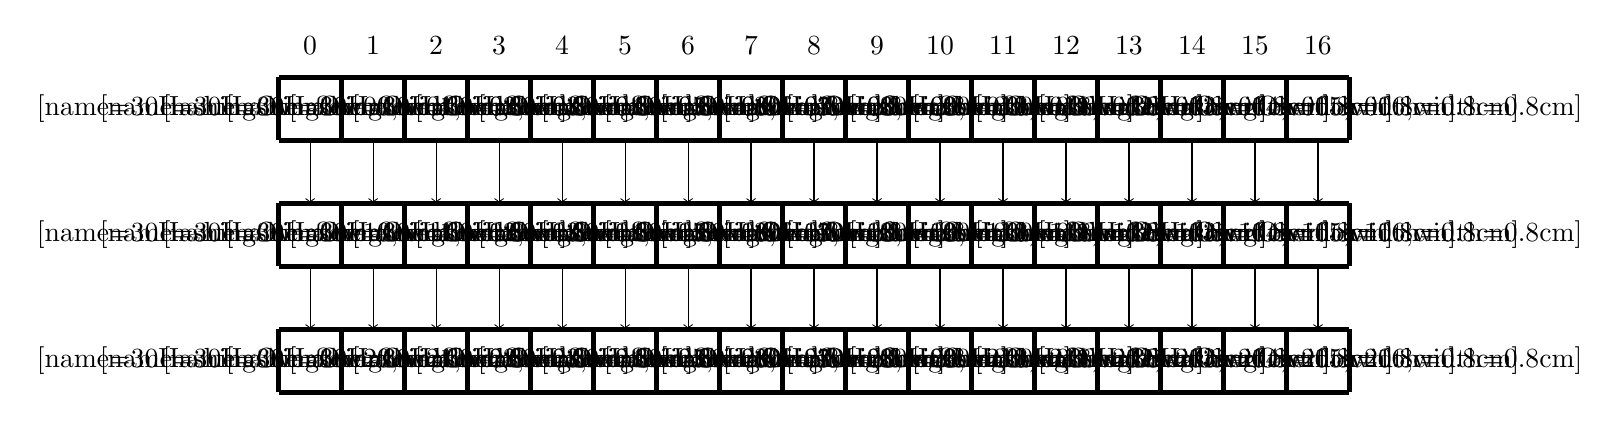
\begin{tikzpicture}
		\draw[step=.8cm, line width=2pt] (0,3.2) grid +(13.6,0.8);
		\draw[step=.8cm, line width=2pt] (0,1.6) grid +(13.6,0.8);
		\draw[step=.8cm, line width=2pt] (0,0) grid +(13.6,0.8);
		\foreach \i in {0,...,16}
		{
			\node at (0.4+0.8*\i, 4.4) {\i};
			\draw [->] (0.4+0.8*\i,3.2) -- (0.4+0.8*\i,2.4);
			\draw [->] (0.4+0.8*\i,1.6) -- (0.4+0.8*\i,0.8);
		}
	
		\foreach \j in {0,...,2}
		\foreach \i in {0,...,16}
		{
			\node at (0.3+0.8*\i, 3.6-1.6*\j) {\TextField[name=30HashingOverflow\j\i,width=0.8cm]{\null}};
		}
	\end{tikzpicture}
\end{beamerText}

\begin{solution}
\begin{multicols}{3}
\begin{enumerate}[a)]
  \item $11 \bmod {17} = 11$
  \item $31 \bmod {17} = 14$
  \item $83 \bmod {17} = 15$
  \item $28 \bmod {17} = 11$
  \item $17 \bmod {17} = 0$
  \item $48 \bmod {17} = 14$
  \item $45 \bmod {17} = 11$
\end{enumerate}
\end{multicols}

	\begin{tikzpicture}
		\draw[step=.8cm] (0,3.2) grid +(13.6,0.8);
		\draw[step=.8cm] (8.8,1.6) rectangle +(0.8,0.8);
		\draw[step=.8cm] (11.2,1.6) rectangle +(0.8,0.8);
		\draw[step=.8cm] (8.8,0.0) rectangle +(0.8,0.8);

\foreach \i in {0,...,16}
{
		\node at (0.4+0.8*\i, 4.4) {\i};
}

		\node at (0.4, 3.6) {17};
		\node at (9.2, 3.6) {11};
		\node at (11.6, 3.6) {31};
		\node at (12.4, 3.6) {83};

		\node at (9.2, 2.0) {28};
		\node at (9.2, 0.4) {45};
		\node at (11.6, 2.0) {48};

		\draw [->] (9.2,3.2) -- (9.2,2.4);
		\draw [->] (9.2,1.6) -- (9.2,0.8);
		\draw [->] (11.6,3.2) -- (11.6, 2.4);
	\end{tikzpicture}
	\end{solution}
